\chapter{Introduction}
\label{chap:introduction}

\section{Semantic Segmentation}
\label{sec:semantic_segmentation}
In recent years, the field of computer vision has undergone rapid advancements, largely driven by the increasing availability of large-scale annotated datasets, powerful computational resources, and deep learning architectures. Among the many tasks in computer vision, semantic segmentation has emerged as one of the most critical and challenging problems due to its potential applications in numerous real-world domains, such as autonomous driving, medical imaging, remote sensing, robotics, and augmented reality. Unlike simple image classification, which assigns a single label to an entire image, semantic segmentation aims to provide a pixel-level understanding of the visual scene by assigning a semantic label to every pixel in an image as shown in \autoref{fig:semantic_segmentation_example}. This process enables machines to perceive not just the presence of objects, but also their exact spatial extents and boundaries within the visual field.

\begin{figure}[htbp]
    \centering
    \setlength{\tabcolsep}{2pt} % adjust spacing
    \renewcommand{\arraystretch}{0.9}
    % \fbox{ % Add border around the figure
        \begin{minipage}{0.8\textwidth}
            \centering
            % CAMs with class labels on the left
            \begin{tabular}{c c} % first column = label

            % Column headers
            (a) Original Image & (b) Segmented Image \\
            [1mm]
            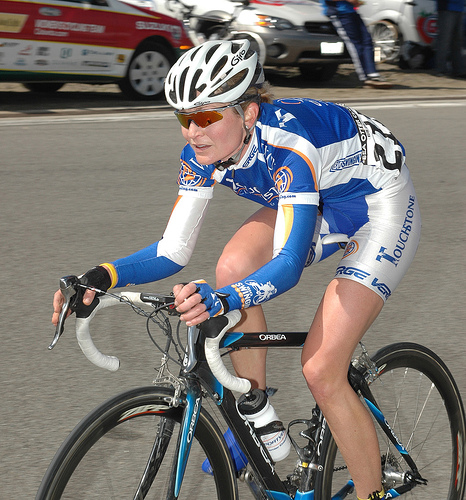
\includegraphics[width=0.45\textwidth,height=0.45\textwidth]{figures/originals/2011_002135.jpg}
            & 
            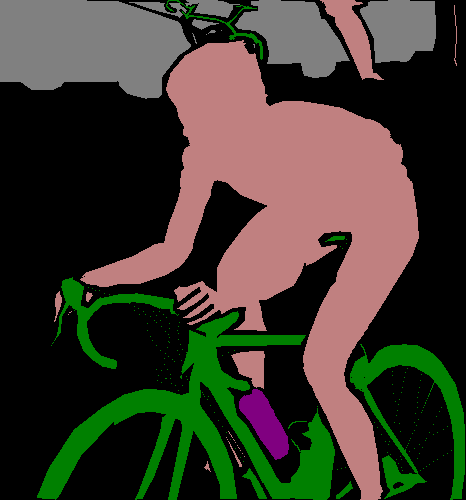
\includegraphics[width=0.45\textwidth,height=0.45\textwidth]{figures/colored_gts/2011_002135.png}
            \\
            \end{tabular}
        \end{minipage}
    % }
    \caption{Original image and Segmented Image.}
    \label{fig:semantic_segmentation_example}
\end{figure}

The goal of semantic segmentation is to transform raw visual data into structured and meaningful representations that align with human perception. For example, in an autonomous driving scenario, semantic segmentation allows a vehicle to distinguish between roads, pedestrians, vehicles, and traffic signs, ensuring both accurate decision-making and safety. In medical imaging, it aids in the precise delineation of organs, tissues, or pathological regions, thereby assisting in diagnosis and treatment planning. Such applications highlight the importance of fine-grained visual understanding, making semantic segmentation a cornerstone task for achieving scene comprehension in artificial intelligence systems.

Traditional approaches to semantic segmentation relied heavily on hand-crafted features and classical machine learning methods such as random forests, support vector machines (SVMs), and conditional random fields (CRFs). While these methods achieved moderate success on specific datasets, they were limited by their inability to capture complex spatial and contextual relationships in images. The breakthrough came with the advent of deep convolutional neural networks (CNNs), which revolutionized the field by automatically learning hierarchical feature representations from data. The introduction of architectures such as Fully Convolutional Networks (FCNs) marked a major milestone, replacing fully connected layers with convolutional ones to enable end-to-end pixel-level prediction. Subsequent models, including U-Net, SegNet, DeepLab, and PSPNet, have further refined this capability by incorporating multi-scale feature extraction, encoder-decoder designs, and attention mechanisms to enhance segmentation accuracy and robustness.

Despite these advances, semantic segmentation still faces several challenges. High-quality pixel-level annotations are expensive and time-consuming to obtain, especially for large datasets. Models must also handle issues such as class imbalance, occlusion, scale variation, and boundary precision, which can significantly affect performance. Furthermore, deep models typically require substantial computational resources, making real-time inference a major concern in resource-constrained environments such as mobile or embedded systems. Recent research has thus explored various directions to address these limitations, including weakly supervised, semi-supervised, and unsupervised approaches that reduce the dependency on dense annotations, as well as lightweight architectures optimized for speed and efficiency.

The increasing focus on semantic segmentation has also sparked interest in integrating it with other vision tasks, such as instance and panoptic segmentation, which aim to provide a more comprehensive understanding of the scene by distinguishing individual object instances. Additionally, combining segmentation with temporal and 3D information, as in video and point cloud segmentation, continues to push the boundaries of scene understanding beyond static 2D imagery.

In summary, semantic segmentation represents a vital step toward achieving full scene understanding in computer vision. By providing detailed, structured, and interpretable representations of visual data, it bridges the gap between low-level pixel information and high-level semantic concepts. This research report explores the principles, methodologies, and recent advancements in semantic segmentation, with particular emphasis on deep learning-based approaches and their applications. Furthermore, it discusses the current challenges and potential future directions that could lead to more efficient, generalizable, and human-like visual perception systems.


\subsection{Fully Supervised Semantic Segmentation}
\label{subsec:fully_supervised}
Fully supervised semantic segmentation represents the traditional and most widely adopted paradigm for training segmentation models. In this approach, models are trained on datasets that contain pixel-level annotations—where every pixel in each training image is manually labeled with its corresponding class. This allows the model to learn precise spatial and contextual relationships between objects and their boundaries. Prominent datasets such as PASCAL VOC, Cityscapes, and ADE20K have played a significant role in advancing research under this framework.

\begin{figure}[htbp]
    \centering
    \fbox{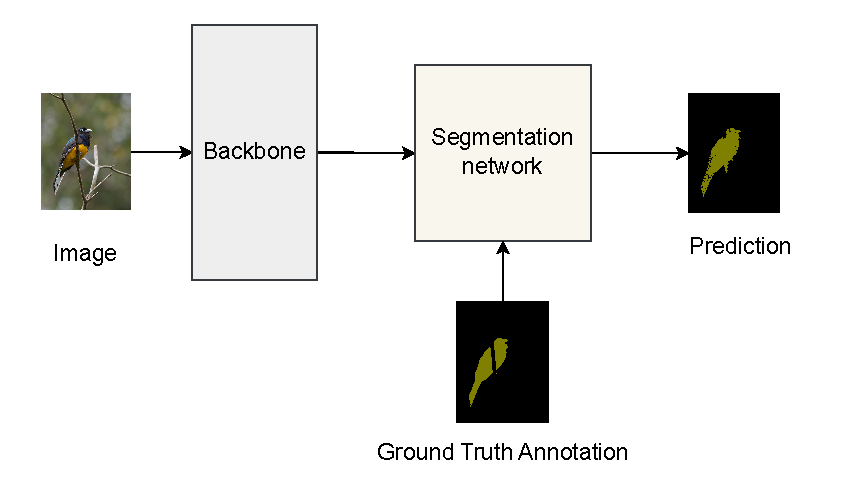
\includegraphics[width=0.9\textwidth]{figures/fsss.pdf}}
    \caption{Pipeline of the fully supervised semantic segmentation framework, where ground-truth pixel-level annotations are used directly to train the segmentation model.}
    \label{fig:fsss}
\end{figure}

In a typical fully supervised setting, a deep convolutional neural network (CNN) or transformer-based architecture learns to map an input image to a dense output map where each pixel corresponds to a predicted semantic label. Models like Fully Convolutional Networks (FCNs), U-Net, SegNet, and DeepLab exemplify the success of this paradigm. These models leverage encoder-decoder designs, skip connections, and multi-scale feature extraction to achieve fine-grained segmentation results. The backbone or the encoder captures global context, while the decoder reconstructs spatial details to produce high-resolution predictions. The pipeline is outlined in \autoref{fig:fsss}.

However, fully supervised learning comes with a major limitation—its dependence on large-scale, densely annotated datasets. The annotation process is not only labor-intensive but also time-consuming and costly, particularly for complex scenes with numerous small or overlapping objects. For instance, annotating a single high-resolution image in the Cityscapes dataset can take several hours. This restricts scalability and makes it difficult to apply such methods to specialized domains like medical imaging or remote sensing, where expert labeling is required. Moreover, fully supervised models may overfit to specific dataset distributions, limiting their generalization to unseen environments. Despite these challenges, fully supervised approaches continue to serve as the benchmark and foundation upon which more flexible and efficient paradigms are built.

\subsection{Weakly Supervised Semantic Segmentation}
\label{subsec:weakly_supervised}
To overcome the data annotation bottleneck in fully supervised learning, weakly supervised semantic segmentation (WSSS) has emerged as a promising alternative. Instead of relying on expensive pixel-level labels, weakly supervised methods train models using weaker forms of supervision, such as image-level labels, bounding boxes, scribbles, or points. The goal is to achieve competitive segmentation accuracy while significantly reducing the labeling effort.

\begin{figure}[htbp]
    \centering
    \fbox{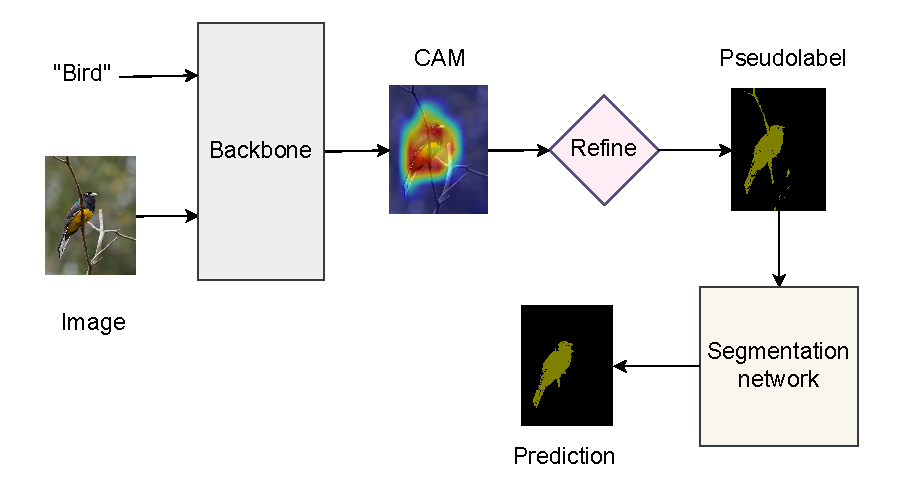
\includegraphics[width=0.9\textwidth]{figures/wsss.pdf}}
    \caption{Pipeline of the WSSS framework illustrating CAM generation, refinement, and pseudo-label creation for segmentation training. Image-level labels serve as weak supervision to generate Class Activation Maps (CAMs), which are subsequently refined into pseudo-labels for training the segmentation network.}
    \label{fig:wsss}
\end{figure}

In WSSS, the central challenge lies in bridging the gap between coarse supervision and fine-grained pixel-level prediction. For example, when only image-level labels are available (e.g., "cat" or "car"), the model must infer which specific regions of the image correspond to each class. Techniques such as Class Activation Maps (CAMs) and region refinement strategies are commonly employed to identify and expand the most discriminative regions into complete object masks. Additionally, saliency maps, pseudo-label generation, and consistency regularization are often used to improve localization accuracy and enforce smoothness in segmentation outputs. The overall pipeline of this process is outlined in \autoref{fig:wsss}.

Weakly supervised approaches are particularly valuable in domains where annotated data is scarce or costly to obtain, such as biomedical imaging or satellite imagery. They also facilitate large-scale training by leveraging vast amounts of web images or unlabeled data. However, because supervision is less precise, WSSS models may suffer from incomplete object coverage, ambiguous boundaries, or noise in pseudo-labels. To mitigate these issues, hybrid approaches that combine weak supervision with semi-supervised or self-supervised learning are increasingly being explored.

Overall, weakly supervised semantic segmentation represents an important step toward scalable and data-efficient learning. By reducing the dependence on exhaustive manual labeling while maintaining reasonable accuracy, it brings the field closer to the ultimate goal of achieving human-like visual understanding with minimal supervision.

\section{Motivation}
\label{sec:motivation}

Semantic segmentation has established itself as a fundamental task in computer vision, with broad applications in areas such as autonomous driving, medical imaging, and robotics. In these domains, a precise pixel-level understanding of the environment is not merely desirable but often critical: for example, safe navigation of self-driving vehicles relies on reliable scene parsing, and accurate delineation of anatomical structures can directly impact medical diagnosis and treatment.

Despite its importance, conventional semantic segmentation has been heavily reliant on fully supervised learning. This paradigm demands large-scale datasets with dense pixel-level annotations, which are costly and labor-intensive to produce. Annotating high-resolution images can take hours per image, and the process remains prone to human error. Beyond annotation effort, fully supervised methods face additional hurdles: (i) class imbalance in real-world datasets often biases models toward dominant categories, (ii) complex scenes with occlusion, lighting variation, and fine structural detail challenge the robustness of predictions, and (iii) models trained on specific datasets frequently fail to generalize across domains due to dataset-specific biases.

These challenges naturally motivate the exploration of weakly supervised semantic segmentation (WSSS). By replacing dense annotations with weaker forms of supervision—such as image-level labels, bounding boxes, or scribbles—WSSS reduces annotation cost while still enabling model training. The key idea is to leverage weak supervision to generate class activation maps (CAMs) and corresponding pseudo-labels, which can then guide the segmentation process. Although CAMs are often coarse or noisy, refinement strategies allow them to approximate dense ground truth, making WSSS a practical compromise between annotation effort and segmentation performance.

The motivation for this research is thus twofold: first, to address the scalability and practicality issues of fully supervised methods, and second, to improve the quality and reliability of WSSS pipelines. By advancing WSSS, we aim to narrow the performance gap with fully supervised segmentation while ensuring that solutions remain feasible for deployment in diverse and data-constrained real-world scenarios.



\section{Problem Statement}
\label{sec:problem_statement}

Weakly Supervised Semantic Segmentation (WSSS) presents a compelling alternative to fully supervised methods by significantly reducing the dependence on costly pixel-level annotations. However, current WSSS techniques rely on Class Activation Maps (CAMs) \cite{cam} generated from image-level labels to identify object regions. While this approach has shown promise, it often falls short in terms of spatial precision and completeness, leading to suboptimal segmentation results.

In the context of WSSS, the challenge lies in effectively leveraging the image-level labels to produce accurate and detailed segmentation maps. The dependence on CAMs, which are typically generated from global features, can result in sparse and coarse activation maps that fail to capture the fine details of object boundaries. This limitation is particularly pronounced when dealing with complex scenes or occlusions, where precise localization is crucial.

Additionally, the refinement techniques applied to these CAMs often fail to fully leverage the rich affinity information inherent in modern transformer architectures. Consequently, the resulting pseudo-labels lack the spatial precision required for high-quality segmentation, ultimately impacting the overall performance. This highlights the need for more robust backbone architectures capable of effectively capturing both local and global features, as well as advanced CAM refinement strategies to narrow the performance gap between weakly and fully supervised segmentation methods.

So, keeping in mind the above challenges, we aim to develop a weakly supervised semantic segmentation model that can effectively leverage image-level labels to produce accurate and detailed segmentation maps. Our approach will focus on enhancing the spatial precision and completeness of the generated CAMs.

\section{Challenges of WSSS}
\label{sec:challenges_of_wsss}

While weakly supervised semantic segmentation (WSSS) reduces the annotation burden compared to fully supervised methods, it introduces its own set of challenges:

\begin{itemize}
    \item \textbf{Incomplete Object Localization:} Class activation maps (CAMs) derived from image-level labels typically highlight only the most discriminative regions, leaving large portions of the object unlabeled.
    \item \textbf{Noisy Pseudo-labels:} The process of refining CAMs into pixel-level labels often introduces noise and errors, which can propagate during training and degrade performance.
    \item \textbf{Boundary Precision:} Weak supervision lacks explicit boundary cues, making it difficult to segment fine object details and separate adjacent instances accurately.
    \item \textbf{Background Confusion:} Without strong pixel-level supervision, models often misclassify diverse background regions as foreground, or vice versa.
    \item \textbf{Multi-class Co-occurrence:} In scenes containing multiple objects, weak labels struggle to capture clear distinctions, leading to overlapping or missing class activations.
    \item \textbf{Class Imbalance:} Underrepresented classes may not produce strong activations in CAMs, resulting in poor segmentation for rare categories.
    \item \textbf{Dependence on External Cues:} Many WSSS methods rely on saliency maps or additional priors to improve CAMs, but these external cues may be dataset-specific and limit generalization.
\end{itemize}

Addressing these challenges is crucial for advancing WSSS methods toward practical applications where annotation resources are limited.


\section{Contribution}
\label{sec:contribution}

In this work, we make the following key contributions:

\begin{itemize}
    \item We explore the use of the UniCL framework \cite{vl_unicl} with a Swin Transformer backbone \cite{transformer_swin} to enhance CAM generation, leveraging Swin's ability to capture both local fine details and global context through its hierarchical structure.
    \item We adapt the affinity-based CAM refinement technique from WeCLIP \cite{wsss_frozen_clip} to the Swin Transformer backbone by computing pixel affinities from Swin's hierarchical features, allowing the refinement to propagate class activations effectively despite the absence of a global attention map.
    \item We integrate a Pixel-Adaptive Refinement Module (PAR) \cite{wsss_afa_affinity_from_attention} that incorporates both color and spatial information, further refining the pseudo-labels and enhancing boundary accuracy.
    \item We integrate the refined CAMs and Pixel-Adaptive Refinement into the standard WSSS training pipeline, training the model to leverage these improved pseudo-labels for better segmentation performance.

\end{itemize}

\section{Organization}
\label{sec:organization}

The remainder of this thesis report is organized as follows:

\begin{itemize}
    \item \textbf{Chapter \ref{chap:related-works}: Related Works} provides a comprehensive review of existing literature on semantic segmentation. It discusses fully supervised and weakly supervised methods, key architectures like U-Net, DeepLab, and Vision Transformers, and identifies gaps in current research.

    \item \textbf{Chapter \ref{chap:methodology}: Proposed Methodology} details the proposed approach, including the use of the UniCL framework with a Swin Transformer backbone for CAM generation. It also describes the affinity-based CAM refinement technique and the Pixel-Adaptive Refinement Module (PAR) for pseudo-label generation and segmentation refinement.
    \item \textbf{Chapter \ref{chap:results-discussion}: Results and Discussion} presents the experimental setup, quantitative and qualitative analysis, including per-class performance, visualizations of CAMs and segmentation masks, ablation study, interpretation of results, discussion of limitations and challenges, and key findings. Additionally, it covers other explored approaches and insights gained from them.

    \item \textbf{Chapter \ref{chap:conclusion}: Conclusion} summarizes the study’s contributions and major insights, emphasizing the broader implications of the findings. It also outlines potential future research directions.
\end{itemize}

This structure ensures a logical flow, starting from the foundational concepts and related works, progressing through the proposed methodology, and concluding with the results, discussions, and supplementary materials.

